\section{Challenges}\label{sec:challenges}

Politou et al. \cite{Politou2017} discussed most of the challenges in smartphone affective research which covers \emph{privacy}, \emph{data misuse}, \emph{trust and engagement}, \emph{multimodal fusion}, \emph{resource constraints}, \emph{affect modelling and representation}, \emph{cultural differences} and \emph{system building costs}. From the technique prespective in this paper mainly focused, challenges and limitations can be shrink to the following sections.

\subsection{Impermeable Emotions}

The primary limitation of traditional affective computing research refers to as impermeable emotions\cite{picard2003affective}. Impermeable emotions is broad, with many of these modalities being inaccessible (e.g., blood chemistry, brain activity, neurotransmitters), and many others being too non-differentiated. This makes it unlikely that collecting the necessary data will be possible or feasible in the near. 

There is a time to express emotion, and a time to forbear; a time to sense what others are feeling and a time to ignore feelings. In every time, human need a balance when they express their emotions, and this balance is missing in computing. Figure~\ref{fig:emotions} illustrates a map of human emotions.

In most cases, researches feel positive and argue that impermeable emotions can be expressed explicitly in other expressed Emotions\cite{parkinson1995ideas} and implicity emotions are trivial and not important for most of the case of affective computing application when we need a emotion state \cite{Zhang2014}. However, impermeable emotions still a open problem and challenges in affective computing research area.

\begin{figure}[htb]
    \centering
    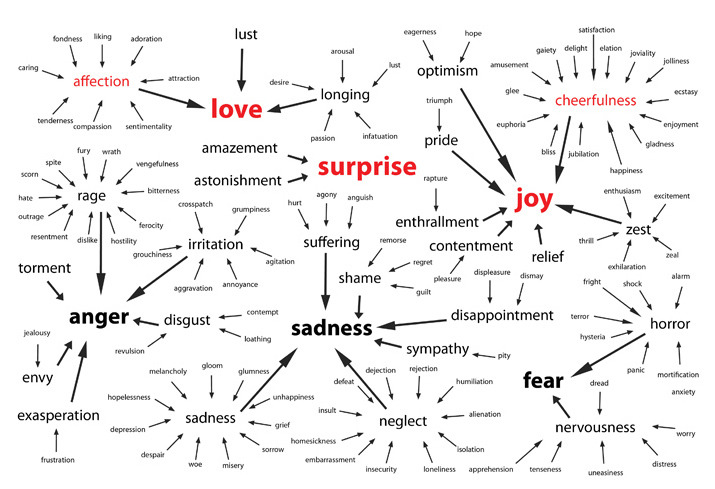
\includegraphics[width=3.5in]{emotion-map}
    \caption{A map of human emotions. Image from\cite{emotionmap}.}
    \label{fig:emotions}
\end{figure}


\subsection{Continious Understanding}

Emotions are instantaneous. Continuous emotion state understanding is much more challenge since its not related to external emotion but also related to internal emotions, various emotions can be expressed as a map \textit{(see Figure~\ref{fig:emotions})}.

Most of the researches we introduced in privous section are trated emotion inferring problem as a classification problem, whereas the human emotions are always passive and instantaneous. People's expression of emotion is so idiosyncratic and variable, that there is little hope of accurately recognizing an individual’s emotional state from the available data sometime. 

\subsection{Context Specific Models}

A potential ethical limitation in research studies comes from the fact that perceptions of emotions and personality are not universal but they are highly dependent on the mobile application context \cite{Gao2012, Shah2015, bhattacharya2017predictive, Tikadar2017} as well as the cultural differences between humans \cite{mesquita1992cultural, masuda2008placing, gendron2014perceptions}. According to these perspectives, a reasonable challenge is how an affective recognition model should be designed and built in a application and cultural transparent way.

\subsection{Lack of Computation Resources}

Affective information, like emotions and personality traits, can
be inferred from various communication channels such as facial and body expressions, speech, text and embedded smartphone sensors or biosensors. 
However, a challenging issue that impacts the effectiveness of affective technology is the fusion of these modalities for building competent multimodal affective recognition systems. 
A multimodal affective recognition system is a system that, via multiple inputs, retrieves affective information from various types of sources and associates input data with a finite set of affective states\cite{ganti2011mobile}.

The problems in regard to the implementation of an effective system with multimodal fusion are plenty and they mainly concern the great variations of data in terms of structure and content, the varied velocity of data reception, the different sampling rate and quality of received data and the continuous growing of data size.
Existing complex technical solutions should be implemented in an energy and power saving approach by keeping in mind that mobile phones have limited operation time and processing power. 

Additionally, mobile affective applications should be implemented with a higher portability to address interoperability issues, since mobile devices may not only be equipped with different mobile platforms and operation environments \cite{khan2013mobile}, but with different sensor capabilities as well. Consequently, given the diversity of mobile devices in availability and capabilities, modelling and predicting the energy and processing requirements to accomplish even a particular emotion inferring task remains a complex issue.